\documentclass[11pt,twoside,a4paper]{article}
% http://www-h.eng.cam.ac.uk/help/tpl/textprocessing/latex_maths+pix/node6.html symboles de math
% http://fr.wikibooks.org/wiki/Programmation_LaTeX Programmation latex (wikibook)
%=========================== En-Tete =================================
%--- Insertion de paquetages (optionnel) ---
\usepackage[french]{babel}   % pour dire que le texte est en fran{\'e}ais
\usepackage{a4}	             % pour la taille   
\usepackage[T1]{fontenc}     % pour les font postscript
\usepackage{epsfig}          % pour gerer les images
%\usepackage{psfig}
\usepackage{amsmath, amsthm} % tres bon mode mathematique
\usepackage{amsfonts,amssymb}% permet la definition des ensembles
\usepackage{float}           % pour le placement des figure
\usepackage{verbatim}

\usepackage{longtable} % pour les tableaux de plusieurs pages

\usepackage[table]{xcolor} % couleur de fond des cellules de tableaux

\usepackage{lastpage}

% \usepackage[top=1.5cm, bottom=1.5cm, left=1.5cm, right=1.5cm]{geometry}
% gauche, haut, droite, bas, entete, ente2txt, pied, txt2pied
\usepackage{vmargin}
\setmarginsrb{0.20cm}{0.20cm}{0.20cm}{0.20cm}{15pt}{3pt}{15pt}{3pt}

\usepackage{lscape} % changement orientation page
%\usepackage{frbib} % enlever pour obtenir references en anglais
% --- style de page (pour les en-tete) ---
\pagestyle{empty}

% % % en-tete et pieds de page configurables : fancyhdr.sty

% http://www.trustonme.net/didactels/250.html

% http://ww3.ac-poitiers.fr/math/tex/pratique/entete/entete.htm
% http://www.ctan.org/tex-archive/macros/latex/contrib/fancyhdr/fancyhdr.pdf
% \usepackage{fancyhdr}
% \pagestyle{fancy}
% % \newcommand{\chaptermark}[1]{\markboth{#1}{}}
% % \newcommand{\sectionmark}[1]{\markright{\thesection\ #1}}
% \fancyhf{}
% \fancyhead[LE,RO]{\bfseries\thepage}
% \fancyhead[LO]{\bfseries\rightmark}
% \fancyhead[RE]{\bfseries\leftmark}
% \fancyfoot[LE]{\thepage /\pageref{LastPage} \hfill
	% TITLE
% \hfill 
\includegraphics[width=0.5cm]{img/logo_glider.png} }
% \fancyfoot[RO]{
\includegraphics[width=0.5cm]{img/logo_glider.png} \hfill
	% TITLE
% \hfill \thepage /\pageref{LastPage}}
% \renewcommand{\headrulewidth}{0.5pt}
% \renewcommand{\footrulewidth}{0.5pt}
% \addtolength{\headheight}{0.5pt}
% \fancypagestyle{plain}{
	% \fancyhead{}
	% \renewcommand{\headrulewidth}{0pt}
% }


%============================= Corps =================================
\begin{document}

\setlength\parindent{0pt}

\texttt{http://www.linformaticien.com/actualites/id/30298/qu-est-ce-qui-ne-tourne-pas-rond-dans-les-formations-informatiques.aspx}~\\

\textbf{\LARGE Qu'est-ce qui ne tourne pas rond dans les formations informatiques ?} ~\\

\emph{\small par Margaux Duquesne, le 18 septembre 2013 15:17} ~\\

\textbf{Les jeunes sortant d'{\'e}coles d'ing{\'e}nieurs sont-ils directement employables ? Les formations en informatique propos{\'e}es en France r{\'e}pondent-t-elles vraiment aux besoins des entreprises ? Ces questions {\'e}taient en d{\'e}bat, ce matin, {\`a} la Maison des Polytechniciens {\`a} Paris, alors que l'{\'E}cole 42 de Xavier Niel pr{\'e}pare sa premi{\`e}re rentr{\'e}e. } ~\\

On le r{\'e}p{\`e}te souvent, les formations actuelles ({\'e}cole, universit{\'e}, BTS...) ne sont pas appropri{\'e}es aux attentes des employeurs. Qu'est-ce qui cloche ? Ces formations sont d{\'e}cal{\'e}es, elles n'avancent pas aussi vite que l'{\'e}volution des technologies. Se creuse ainsi un foss{\'e} entre les {\'e}l{\`e}ves et les recruteurs. Et tout le monde est finalement perdant, avec le ch{\^o}mage en toile de fond et des entreprises qui peinent {\`a} trouver la "perle rare". ~\\

\begin{minipage}[ht]{7.00cm}
	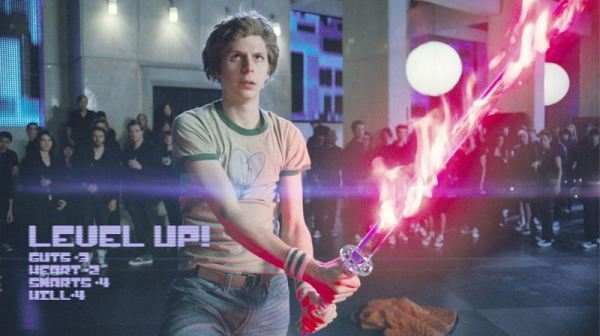
\includegraphics[width=6.95cm]{img/59580392.jpg}
\end{minipage} \hfill \begin{minipage}[ht]{0.65\textwidth}
	Quand d'un c{\^o}t{\'e} une entreprise comme Accenture recherche des candidats qui ont \emph{<<la technique et une bonne connaissance de l'entreprise>>}, comme l'explique Anissa Deal, responsable du d{\'e}veloppement chez Accenture France, Nicolas Sadirac et son {\'E}cole 42 cherchent davantage {\`a} cr{\'e}er des profils de personnes \emph{<<qui se sont {\'e}panouies dans la technologie>>}.  Si ces deux visions semblent diff{\'e}rentes, montrant le foss{\'e} entre l'ancienne {\'e}cole et la rel{\`e}ve, elles ne sont pas non plus incompatibles. Il est tout {\`a} fait possible d'{\^e}tre autodidacte et passionn{\'e} de d{\'e}veloppement, tout en r{\^e}vant depuis de nombreuses d'ann{\'e}es d'int{\'e}grer une structure comme EADS et d'en conna{\^i}tre ainsi les enjeux. %% ~\\
\end{minipage}~\\~\\

\textbf{\large Au secours de l'industrie fran\c{c}aise}~\\

Bien s{\^u}r, de l'autre c{\^o}t{\'e}, les autorit{\'e}s politiques doivent prendre leurs responsabilit{\'e}s car il s'agit bien de prot{\'e}ger ces fili{\`e}res et d'{\'e}viter la fuite des cerveaux. En effet, ces derniers n'h{\'e}siteront pas {\`a} se tourner vers les pays anglo-saxons qui ne demandent pas <<Quels dipl{\^o}mes ont les candidats ?>> mais bien : <<Que savent-ils faire, effectivement, de leurs dix doigts ?>>. C'est en tout cas ce que rappelle Geoffrey Burns, directeur du recrutement, au d{\'e}partement Application Services, chez Capgemini France. ~\\

Le probl{\`e}me vient-il aussi du c{\^o}t{\'e} des entreprises ? Autour de la table, une femme intervient et soul{\`e}ve cet {\'e}tat de fait : \emph{<<Je vois passer toute la journ{\'e}e des offres d'emploi pour des grands groupes comme Airbus. Ils recherchent des candidats qui connaissent D{\'E}J{\`A} tr{\`e}s bien l'entreprise et qu'ils n'auront plus qu'{\`a} installer {\`a} leur nouveau poste. Comment voulez-vous que les jeunes se pensent comp{\'e}tents ?>>}. En r{\'e}ponse, on souligne seulement qu'un candidat doit r{\'e}pondre au maximum de crit{\`e}res d'une annonce, mais ne peut {\'e}videmment pas avoir toutes les qualit{\'e}s demand{\'e}es. Sous-entendu : m{\^e}me si vous ne connaissez pas toute la technologie de l'entreprise par c\oe ur, candidatez. ~\\

Un autre probl{\`e}me est soulev{\'e} aussi : celui de la \emph{<<deuxi{\`e}me partie de carri{\`e}re>>}. Que faire de nos seniors ? <<Chez Accenture, nous les accompagnons pour les aider {\`a} se rediriger vers d'autres m{\'e}tiers car nous avons la chance d'{\^e}tre une grande structure.>> Yaya Sylla, architecte chez Teradata International, explique que l'{\^a}ge moyen de ses collaborateurs a chang{\'e} au fil des ans : \emph{<<Il y a cinq ans, cet {\^a}ge moyen {\'e}tait de 48 ans. Nous avons voulu rajeunir nos {\'e}quipes et en m{\^e}me temps valoriser nos seniors. Ils ont d{\'e}sormais aussi un r{\^o}le de coaching, ils accompagnent les jeunes. Les seniors sont tr{\`e}s recherch{\'e}s, du coup ! Et notre {\^a}ge moyen a baiss{\'e} {\`a} environ 42/43 ans.>>} ~\\

\textbf{\large Collaborer, c'est tricher ?}~\\

\begin{minipage}[ht]{7.00cm}
	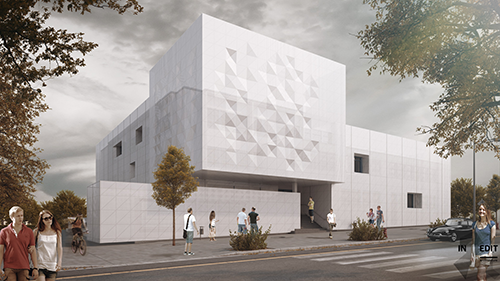
\includegraphics[width=6.95cm]{img/01-Exterieur.png}
\end{minipage} \hfill \begin{minipage}[ht]{0.65\textwidth}
	L'{\'E}cole 42, cr{\'e}{\'e}e {\`a} l'initiative de Xavier Niel, et repr{\'e}sent{\'e}e par Nicolas Sadirac, en est une des r{\'e}ponses, mais pas la seule, comme ils le disent r{\'e}guli{\`e}rement. Elle s'appuie sur le constat alarmant que la France se place au vingti{\`e}me rang dans l'{\'e}conomie num{\'e}rique mondiale. En mars dernier, l'annonce de sa cr{\'e}ation provoque un petit s{\'e}isme dans l'industrie du num{\'e}rique fran\c{c}ais. Certains diront que ce n'est pas suffisant et que l'{\'E}cole 42 ne remplacera jamais un bon vieux dipl{\^o}me d'{\'e}cole d'ing{\'e}nieur, d'autres applaudiront ce pragmatisme et cette volont{\'e} d'emp{\^e}cher ce milieu de tourner en rond. %% ~\\
\end{minipage}~\\~\\

\textbf{\large Deux "piscines" cet {\'e}t{\'e} {\`a} l'{\'E}cole 42}~\\

	Cet {\'e}t{\'e}, les responsables de l'{\'E}cole 42 ont \emph{<<s{\'e}lectionn{\'e}>>} leurs 800 futurs purs-sangs de l'informatique, {\`a} travers l'{\'e}preuve de la \emph{<<piscine>>} : un enfermement d'un mois o{\`u} les candidats r{\'e}alisent de nombreux exercices, de mani{\`e}re intensive. Deux \emph{<<piscines>>} ont {\'e}t{\'e} d{\'e}j{\`a} organis{\'e}es, cet {\'e}t{\'e}, et la derni{\`e}re est en cours. ~\\

\begin{minipage}[ht]{7.00cm}
	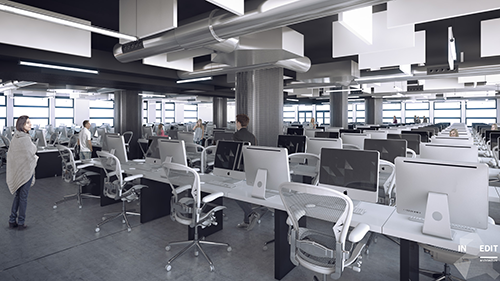
\includegraphics[width=6.95cm]{img/03-Piscines.png}
\end{minipage} \hfill \begin{minipage}[ht]{0.65\textwidth}
	\emph{<<Dans les {\'e}coles traditionnelles, \emph{<<collaborer>>} est assimil{\'e} {\`a} \emph{<<tricher>>}. Nous, nous faisons du travail en groupe, nous produisons collectivement. Cette diversit{\'e} est importante, tout comme permettre d'apporter ses propres id{\'e}es dans un syst{\`e}me g{\'e}n{\'e}rateur d'id{\'e}es.>>}, indique Nicolas Sadirac. Il conclut : \emph{<<Ce qui nous int{\'e}resse est davantage l'{\'e}volution pour d{\'e}celer ce qu'est capable d'acqu{\'e}rir une personne. C'est un m{\'e}tier d'artiste, nous cherchons des talents.>>} Les responsables de l'{\'E}cole 42 sont {\`a} all{\'e}s {\`a} la rencontre des patrons du Medef, derni{\`e}rement. Tous rapportent le m{\^e}me probl{\`e}me : comment migrer vers l'{\'e}conomie num{\'e}rique ? Vaste programme. En attendant, les premiers {\'e}l{\`e}ves de l'{\'E}cole 42 commenceront les formations atypiques en novembre prochain. %% ~\\
\end{minipage}~\\~\\

\end{document}
